% This is style of APS journal, physicists should aim to use it
\documentclass[prl,12pt,notitlepage,aps,onecolumn,superscriptaddress]{revtex4-1}

%---------------------------------------------------------------
\usepackage{listings} % allow to include nicely formated listings
\usepackage{xcolor}   % we can add and use colors
\usepackage{fullpage} % default article style is to greedy about margins
\usepackage{graphicx} % REQUIRED TO WORK WITH FIGURES
\usepackage{amsmath,amssymb} % much better math and equation handling
\usepackage{booktabs}
\usepackage{float}
%---------------------------------------------------------------

\begin{document}
%---------------------------------------------------------------
\title{Lab 05 Report}
\author{William Laney \& Karen Ficenec}
\date{October 11, 2016}
\maketitle

\section{Group Member Roles}
Resource Manager (collected and tested componets): William and Karen

Hardware Specialist (assembled the circuit): William and Karen

Programer: William and Karen

QA Specialist William and Karen

\section{Inital set up and testing}
We began this lab by connecting the MCP3002 anolgue to digital convertor (ADC) to the raspbeery pi using SPI. We used GPIO 08 as the chip select pin. This desgine came from the Lab 5 instructions. To confirm that the ADC was working corectly, and to discover the bounds of the device we put a DC voltage into input 1 of the MCP3002 and tied input 2 to ground. We then varied the input voltage from 0 to near 3.3V. We did not go over 3.3V because this was the voltage used to power the device, and thus the upper rail. The results of this can be seen in table 1. The plot seen in figure 1 shows the percent error between the voltage input messured by a digital multi meter and the input voltage messured by the ADC. From this we learned that the MCP3002 is less precies when the voltage is near ground, and gains presion until the voltage is about 0.25V, then the it stays constant. This is expected because at low voltages the messured voltage is closer to the noise in the system. We belive that if we placed a capictor to ground at the Vin pin we could increase the pression of readings at lower voltages.

% Table generated by Excel2LaTeX from sheet 'Sheet1'
\begin{table}[h]
  \centering
  \caption{DC Voltage Readings}
    \begin{tabular}{c|c|c}
    \toprule
    Expected & Observed & Percent Error \\
    \midrule
    0.005 & 0.006 & 0.2 \\
    0.25  & 0.251 & 0.004 \\
    0.513 & 0.512 & 0.001949318 \\
    0.723 & 0.728 & 0.006915629 \\
    1.042 & 1.044 & 0.001919386 \\
    1.265 & 1.267 & 0.001581028 \\
    1.542 & 1.54  & 0.001297017 \\
    1.738 & 1.74  & 0.001150748 \\
    2.102 & 2.104 & 0.000951475 \\
    2.275 & 2.275 & 0 \\
    2.539 & 2.539 & 0 \\
    2.799 & 2.8   & 0.00035727 \\
    3.061 & 3.062 & 0.000326691 \\
    3.188 & 3.184 & 0.001254705 \\
    \bottomrule
    \end{tabular}%
  \label{tab:addlabel}%
\end{table}%

\begin{figure}[h]
\begin{center}
\includegraphics[width=.5\columnwidth]{plot.png}
\end{center}
\caption{\label{fig:pic} Percent error graph}
\end{figure}

\section{Creating a Scope}
Next we wrote code that would recored a series of data points and plot them. This allows use to see how voltage vaires at time and look at wave forms. We found through expermentation that recording about 1000 data points at the maximum sampling frequency of the Pi led to the best results. In addion to recoding and ploting data we created code that would use an extrenal triger to begin the data sampling. We used an interup servious routine that waited for a rising edge to trigger. We then connected the TTL to the interup tpin and used this to trigger our scope. On a sine wave the TTL sends a high pulse at the bigging of the rising part of the sign wave. Due to speed constraints of the pi this caused it to begin sampling data normaliy somewhere near the peak of the sign wave. The code we used, with the modification dicues below for speed improvents, in the scope can be seen in listing 1, in the apendix. A picture of our set up can be seen in figure 2.

\begin{figure}[h]
\begin{center}
\includegraphics[width=.5\columnwidth]{cir_pic.jpg}
\end{center}
\caption{\label{fig:pic} Scope circuit}
\end{figure}

Now that we had a working scope with an extral trigger we started to try to determine the maximum frequency it could accuretly recored. We found that the maximum frequncy was about 350Hz. Figures 3, 4, and 5 show 40hz 350hz, and 1.08kz respectivly. These figures show that as the frequency of the input goes up the pi can no longer smaple enough points to make a smoth curve. While at the higher frequencies it may still be possible to accurely calculate the frequency of the wave we do not belive that this corospoends to an opeating scope because no information can be provided about the wave form of the input.

\begin{figure}[h]
\begin{center}
\includegraphics[width=.5\columnwidth]{40sin.png}
\end{center}
\caption{\label{fig:pic} 40hz}
\end{figure}

\begin{figure}[h]
\begin{center}
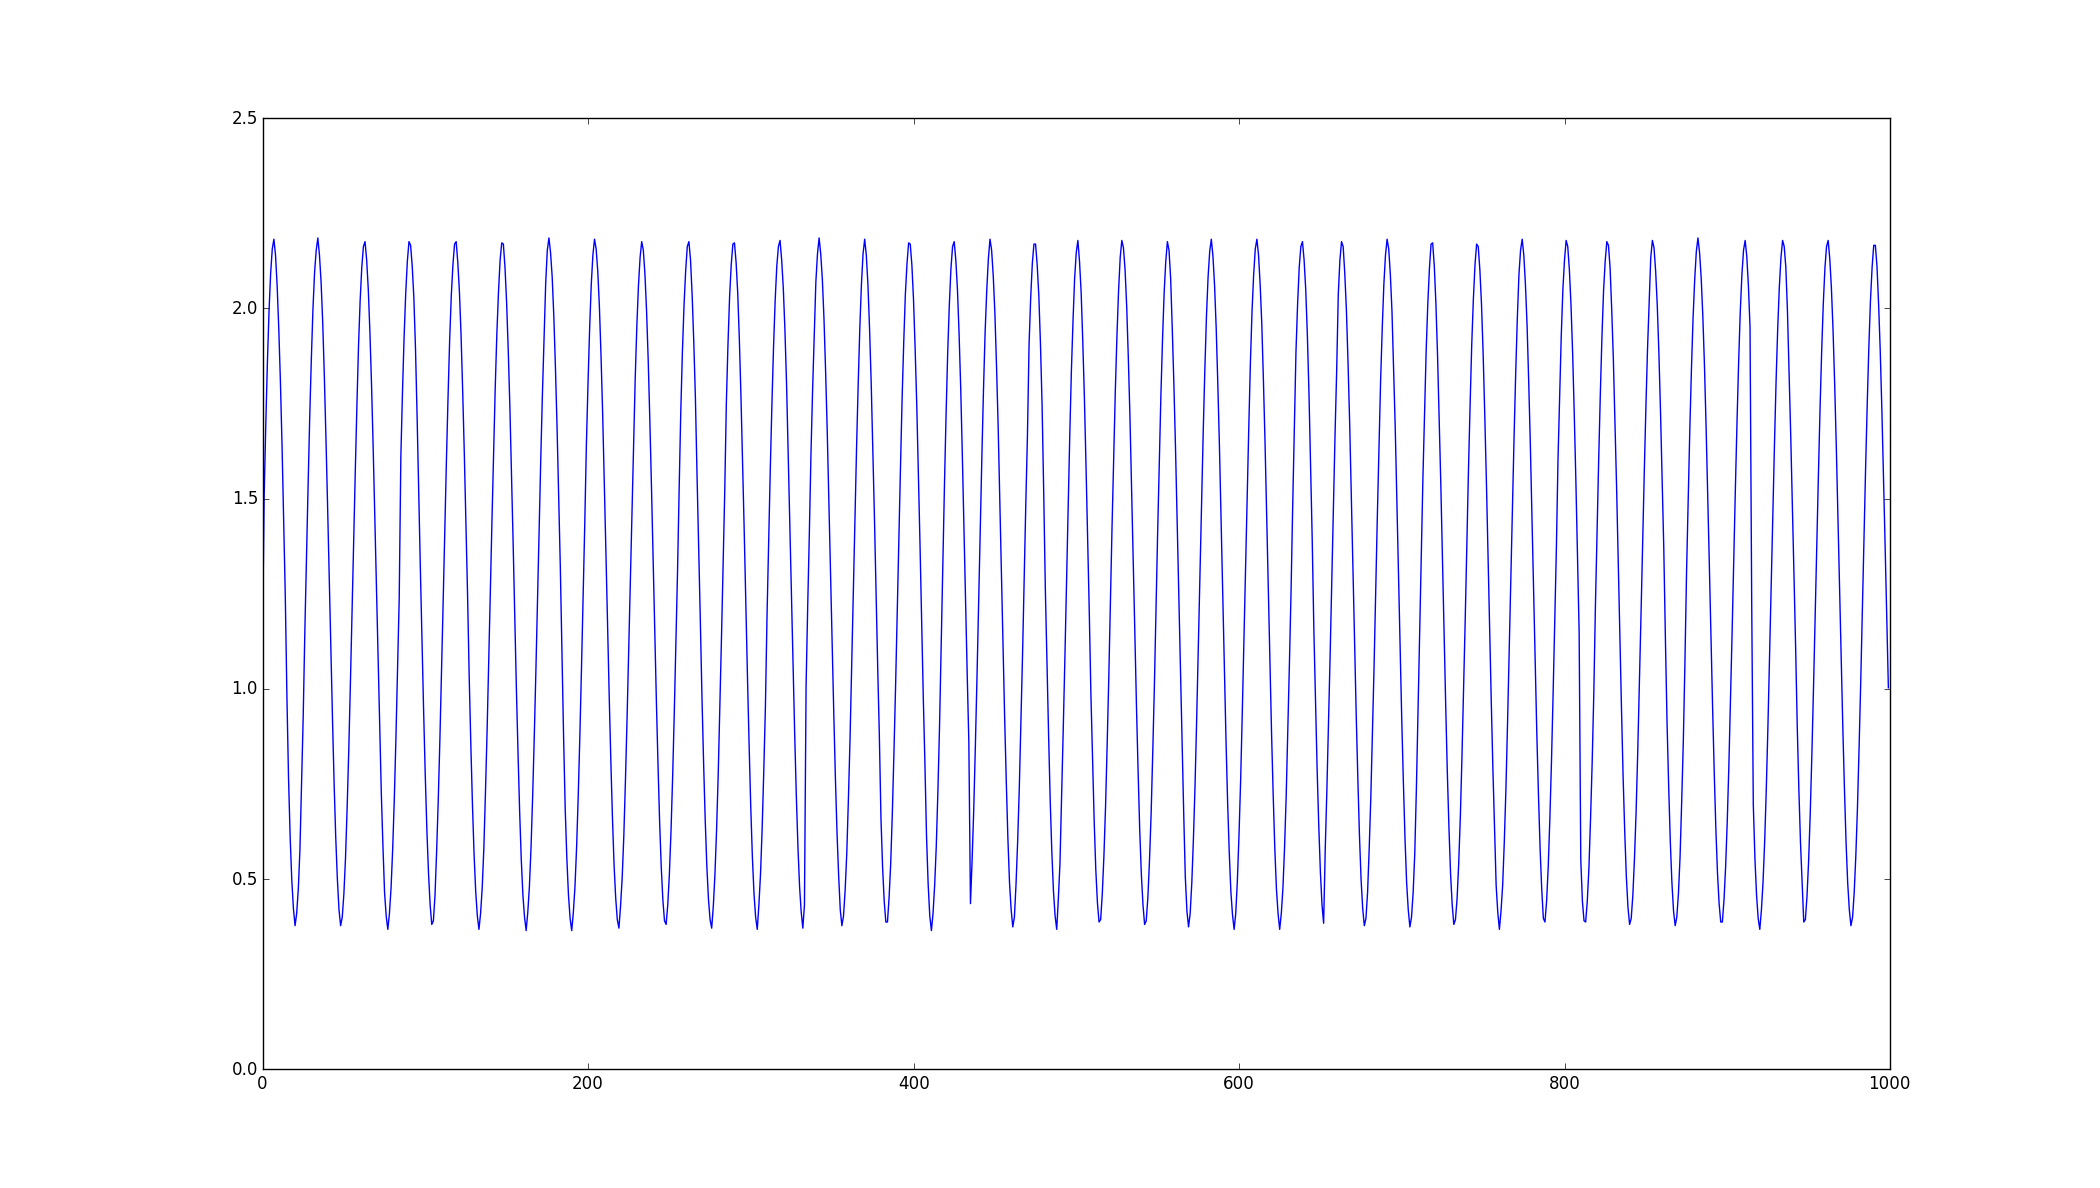
\includegraphics[width=.5\columnwidth]{350_max_freq.png}
\end{center}
\caption{\label{fig:pic} 350Hz}
\end{figure}

\begin{figure}[h]
\begin{center}
\includegraphics[width=.5\columnwidth]{1k08.png}
\end{center}
\caption{\label{fig:pic} 1.08kHz}
\end{figure}

With this maximum found we tryed to imporve the scope. To do this we began to preallocate memory for storing the data points. In our orginal code each data point was added on to the end of a list in each iteration of the loop. This meant that each loop iteration the size of the list changed and the system had to change memory allocation to accomidate this. By creating a list of summy values before the loop and then replacing the dummy values with real data the sytem does not need to change memory allocation with every interation. This lead to us seeing a better looking wave form at 350Hz, as can be seen in figure 6.

\begin{figure}[h]
\begin{center}
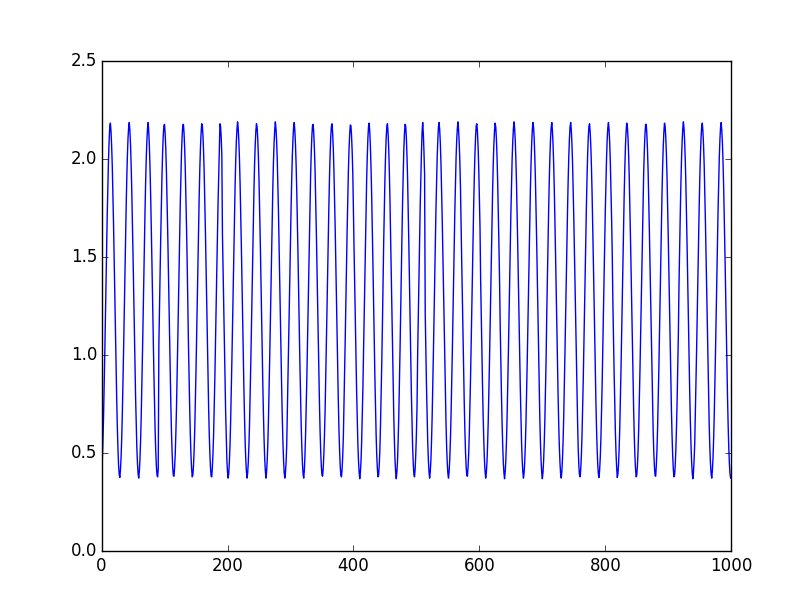
\includegraphics[width=.5\columnwidth]{350_array_good.png}
\end{center}
\caption{\label{fig:pic} 350Hz with memory pre allocation improvments}
\end{figure}


\end{document}